\documentclass[12pt]{article}
\usepackage{array}
\usepackage{amsmath}
\usepackage{mathtools}
\usepackage{gensymb}
\usepackage{graphicx}
\usepackage{float}
\usepackage{caption}

\allowdisplaybreaks

\begin{document}
    \title{Coefficient of Kinetic Friction Between an Air Track and Cart}
    \author{Ryan Coyne and Patrick Browning}
    \maketitle
    \section{Abstract}
        The coefficient of kinetic friction between an air track and cart, \(\mu\), was measured using a modified Atwood machine with a pulley that can measure rotational motion. The coefficient of kinetic friction was measured to be (\(0.0012 \pm 0.0071\)).
    \section{Introduction}
        The formula
        \begin{equation*}
            a = g - \frac{(1+\mu)g}{M}m_1
        \end{equation*}
        can be used to find the acceleration of the masses in a modified Atwood machine, where \(M\) is the sum of the masses and \(m_1\) is the mass resting on the surface. If \(M\) is kept constant when \(m_1\) changes by adding any mass that is removed from \(m_1\) to \(m_2\) or adding mass to \(m_1\) only if it is taken from \(m_2\), then the acceleration is proportional to \(m_1\).
        
        When \(a\) is proportional to and plotted vs \(m_1\), \(g\) is the intercept of the \(a\) axis. In the case of this lab \(g\) will not be 9.8 m/\(\mathrm{s}^2\) because we are not using an ideal pulley and string which these do not exist in the real world. Unlike an ideal pulley and string ours have mass, friction, and elasticity which will lower the acceleration so instead of \(g\) we will use \(g_\mathrm{eff}\) which we can find from the intercept of the graph of \(a\) vs \(m_1\).  The slope of the resultant line when \(a\) is plotted vs \(m_1\) is showing in the equation for acceleration to be 
        \begin{equation*}
            S = - \frac{(1+\mu)g_\mathrm{eff}}{M}
        \end{equation*} 
        from which we can find the coefficient of friction.
    \section{Procedure}
        The mass of a cart was measured using a triple beam balance. The cart was place on an air track which was placed on a table. The track was leveled by turning it on and adjusting the heights of the legs until the cart remained in place. Once level the track was turned off. A pulley rotational motion sensor was attached to a rod which was clamped to the table. A string was hooked to the cart and placed over the pulley. The pulley was then lined up with the cart so that the string was parallel to the track. Two fifty gram and five twenty gram weights were attached to the cart. A fifty gram hook which the twenty gram weights could be attached to was hung from the end of the string not attached to the cart. The motion sensor was connected to a laptop to record the data. Six trials were conducted with one twenty gram weight moved from the cart to the hook between each trial.
        \begin{figure}[H]
            \centering
            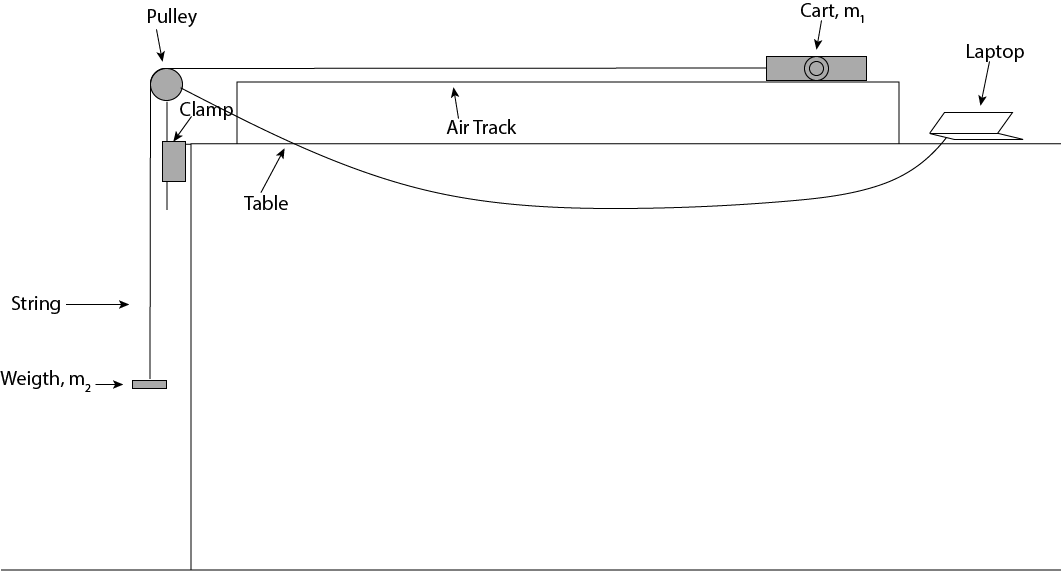
\includegraphics[width=\linewidth]{Experimental Setup.png}
            \caption{Experimental Setup}
        \end{figure}
    \section{Data}
        \begin{center}
            \begin{tabular}{c|cc}
                Trial & \(m_1\) kg & \(a\) (m/\(\mathrm{s}^2\))\\
                \hline
                1 & 0.39971 & 1.03585\\
                2 & 0.37971 & 1.4572\\
                3 & 0.35971 & 1.8818\\
                4 & 0.33971 & 2.3036\\
                5 & 0.31971 & 2.7007\\
                6 & 0.29971 & 3.1459
            \end{tabular}\\
            Table 1. Dependance of acceleration on mas \(m_1\).\\[14pt]
            \begin{tabular}{c|c} 
                Trial & \(M\) (kg)\\
                \hline
                1 & 0.44963\\
                2 & 0.44979\\
                3 & 0.44965\\
                4 & 0.44977\\
                \hline
                \(\overline{M}\) & 0.44971\\
                \(\sigma_M\) & \(8.1\mathrm{x}10^{-5}\)
            \end{tabular}\\
            Table 2. Total mass.
        \begin{figure}[H]
            \centering
            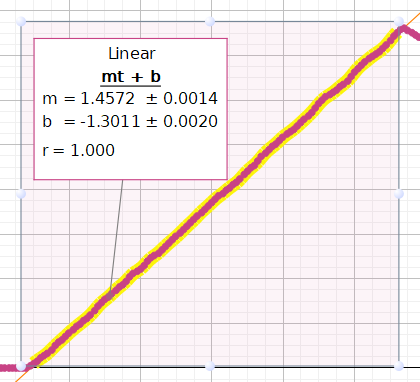
\includegraphics{Velocity vs Time.png}
            \caption{Sample plot of velocity vs time with fit to determine acceleration.}
        \end{figure}
        \begin{figure}[H]
            \centering
            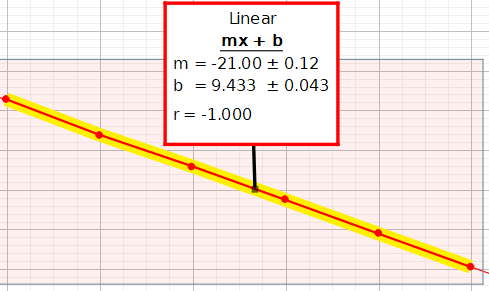
\includegraphics{Acceleration vs m1.png}
            \caption{Plot of \(a\) vs \(m_1\) with fit to find slope and intercept with error.}
        \end{figure}
    \end{center}
    \section{Calculations}
        \begin{figure}[H]
            \centering
            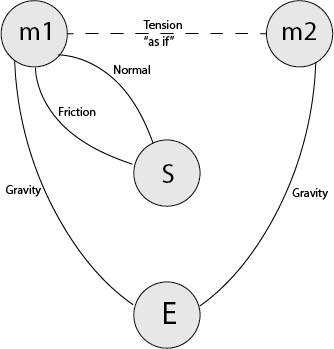
\includegraphics[height=0.4\textheight]{Interaction Diagram.png}
            \caption{Interaction Diagram}
        \end{figure}
        \begin{figure}[H]
            \centering
            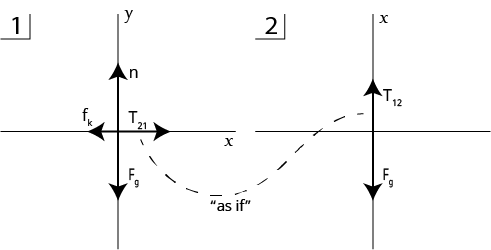
\includegraphics[width=\linewidth]{Free Body Diagram.png}
            \caption{Free Body Diagram}
        \end{figure}
        \begin{alignat*}{3}
            (1)~
            &&T_{12} &= m_2g - m_2a_{2x}\\
            &&T_{21} &= m_1a_{1x}+\mu m_1g\\
            &&T_{12} &= T_{21}=T\\
            &&a_{1x} &= a_{2x} = a\\
            &&m_2g-m_2a &= m_1a+\mu m_1g\\
            &&m_2a+m_1a &= m_2g-\mu m_1g\\
            &&a &= \frac{m_2g-\mu m_1g}{m_1+m_2}\\
            &&&= g\frac{m_2-\mu m_1}{m_1+m_2}\\
            &&M &= m_1 + m_2\\
            &&m_2 &= m_1 - M\\
            &&a &= g\frac{M-m_1-\mu m_1}{M}\\
            &&&= g\frac{M-(1+\mu)m_1}{M}\\
            &&&= g - g\frac{(1+\mu)m_1}{M}\\
            &&&= g\left(1 - \frac{(1+\mu)m_1}{M}\right)\\
            (2)~
            &&\frac{\sigma_M}{\overline{M}} & = \frac{8.16497\mathrm{x}10^{-5}}{0.44971}\\
            &&& = 0.01816\%\\
            &&\frac{\sigma_S}{\overline{S}} & = \frac{0.12}{21}\\
            &&& = 0.57143\%\\
            &&\frac{\sigma_{g_\mathrm{eff}}}{\overline{g_{\mathrm{eff}}}} & = \frac{0.0433}{9.43}\\
            &&& = 0.45917\%\\
            (3)~
            && \overline{\mu} &= -\frac{SM}{g_\mathrm{eff}}-1\\
            &&& = -\frac{-21 \cdot 0.44971}{9.433}-1\\
            &&& = 0.0012\\
            (4)~&&\mu_S &= -\frac{(S+\sigma_S)M}{g_{\mathrm{eff}}}-1\\
            &&& = -\frac{(-21.0 + 0.12)~\mathrm{m}/(kg\mathrm{s}^2) \cdot 0.450~\mathrm{kg}}{9.433~\mathrm{m}/\mathrm{s}^2}-1\\
            &&& = -\frac{(-20.88)~\mathrm{m}/(kg\mathrm{s}^2) \cdot 0.44971~\mathrm{kg}}{9.433~\mathrm{m}/\mathrm{s}^2}-1\\
            &&& = -\frac{9.396~\mathrm{m}/\mathrm{s}^2}{9.433~\mathrm{m}/\mathrm{s}^2}-1\\
            &&& = -0.00425\\
            && \mu_{g_\mathrm{eff}} &= -\frac{SM}{g_{\mathrm{eff}}+\sigma_{g_\mathrm{eff}}}-1\\
            &&& = -\frac{-21~\mathrm{m}/(kg\mathrm{s}^2 \cdot 0.44971~\mathrm{kg}}{(9.433 + 0.043)~\mathrm{m}/\mathrm{s}^2}-1\\
            &&& = \frac{9.44391~\mathrm{m}/\mathrm{s}^2}{9.476~\mathrm{m}/\mathrm{s}^2}-1\\
            &&& = -0.00339\\
            && \sigma_\mu &= \sqrt{(\mu_S - \overline{\mu})^2 + (\mu_{g_\mathrm{eff}} - \overline{\mu})^2}\\
            &&& = \sqrt{(-0.00425-0.00115)^2 + (-0.00339-0.00115)^2}\\
            &&& = \sqrt{(-0.004543)^2+(-0.0054042)^2}\\
            &&& = \sqrt{0.0000206+0.0000292}\\
            &&& = \sqrt{0.0000498}\\
            &&& = 0.0071\\
        \end{alignat*}
    \section{Conclusion}
    No measurements had greater error than was to be expected from random error based on the precision of the balance. The exact precision of the pulley rotational motion sensor is unknown but the measurements from the pulley seem to be reasonable. The value for \(g_\mathrm{eff}\) was lower than 9.8 m/\(\mathrm{s}^2\) as expected. The coefficient of friction was within a standard deviation of zero which was also expected.
\end{document}